\subsection{Модификация закона Амдала (по проф. Бухановскому)}

В реальных вычислительных системах ОС тратит ресурсы на создание и удаление новых потоков. Время, затраченное на эти операции не учитывается в законе Амдала. Параллельное ускорение $S(p)$ зависит от количества ядер и доли распараллеливаемых операций, но не зависит от количества последних. Выведем формулу в которой количество операций для которых необходимо создать поток будет учитываться.

Пусть $N$ -- количество распараллеливаемых операций, $M$ -- количество нераспараллеливаемых операций, $t_c$ -- время выполнения одной операции, $p$ -- количество вычислителей(ядер), $T_i$ -- время выполнения программы при использовании $i$ параллельных потоков на $i$ вычислителях, $\alpha$ -- некий масштабирующий коэффициент, инкапсулирующий в себе количество времени, требуемого на создание, удаление потока и прочие накладные операции. 
По формуле~\eqref{AmdalSFromP:equation}, $S(p) = {T_1} / {T_p}$.

Найдем сначала $T_1$. Так как это код выполняется линейно, то время затраченное на его выполнение будет равно количеству операций помноженному на время выполнения одной операции: $T_1 = t_c \cdot (N + M)$.

Время выполнение распараллельнной программы $T_p$ включается в себя время на создание потока: $t_c \cdot \alpha \cdot (p - 1) \cdot N$ (нужно создать $(p - 1)$ новых потоков, так как главный поток уже создан и для каждого затратить какое-то время $\alpha$), время работы распараллеливаемоего кода на всех ядрах: $(t_c \cdot N) / {p}$ и время работы нераспараллеливаемого кода $t_c \cdot M$. Итого, разделив $T_1$ на $T_p$, получим формулу закона Амдала по проф. Бухановскому:

\begin{equation}
    \label{AmdalBuhunovsky:equation}
    S(p,N) = \frac{T_1}{T_p} = \frac{N + M}{\alpha \cdot (p - 1) \cdot N + \displaystyle\frac{N}{p} + M}
\end{equation}

Из формулы~\eqref{AmdalBuhunovsky:equation} видно, что с ростом количество ядер после определенного предела $S(p,N)$  не будет расти как в законе Амдала, так как будет тратиться много времени на создание новых потоков. На рисунке~\ref{GraphAmdalBuhunovsky:image} наглядно видно, что $S(p,N)$ уменьшается при большом количестве потоков и становится заметно меньше $S(p)$ по Амдалу даже при небольшом значении $\alpha$.

\begin{figure}[H]
    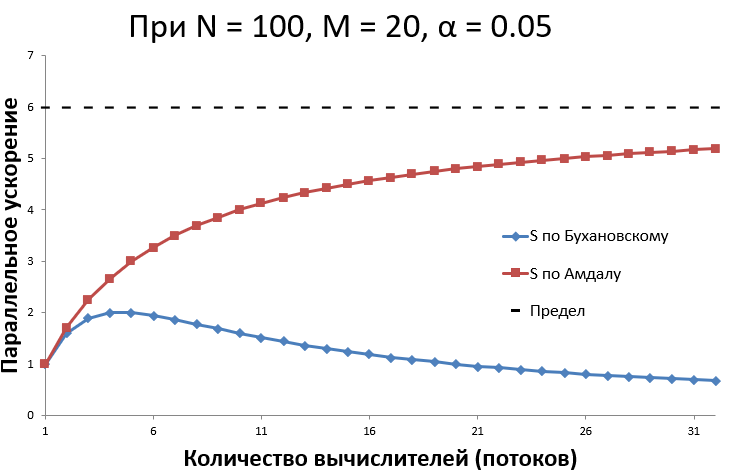
\includegraphics[width=\linewidth]{GraphAmdalBuhunovsky}
    \caption{График зависимости параллельного ускорения от количества потоков}
    \label{GraphAmdalBuhunovsky:image}
\end{figure}
